\documentclass[aspectratio=169, 10pt]{beamer}
\usetheme{Madrid}
\usecolortheme{whale}
\setbeamertemplate{navigation symbols}{}
\setbeamertemplate{footline}[frame number]

\usepackage[utf8]{inputenc}
\usepackage[T1]{fontenc}
\usepackage{amsmath,amssymb,amsfonts}
\usepackage{booktabs}
\usepackage{tabularx}
\usepackage{tikz}
\usetikzlibrary{shapes.geometric, arrows.meta, positioning, calc}

\definecolor{navyblue}{RGB}{18, 52, 99}
\definecolor{accentblue}{RGB}{32, 102, 178}
\definecolor{darkred}{RGB}{175, 35, 35}
\definecolor{darkgreen}{RGB}{25, 120, 60}
\definecolor{softgray}{RGB}{242, 245, 250}

\setbeamercolor{structure}{fg=navyblue}
\setbeamercolor{frametitle}{bg=navyblue, fg=white}
\setbeamercolor{title}{bg=navyblue, fg=white}
\setbeamercolor{block title}{bg=accentblue, fg=white}
\setbeamercolor{block body}{bg=softgray, fg=black}
\setbeamercolor{block title alerted}{bg=darkred, fg=white}
\setbeamercolor{block body alerted}{bg=red!6, fg=black}
\setbeamercolor{block title example}{bg=darkgreen, fg=white}
\setbeamercolor{block body example}{bg=green!6, fg=black}

\title[SemEval-2027 Task 11: PV-VAKRA]{\textbf{Plan-and-Verify Agent with Schema-Grounded Tool Retrieval and Policy Guardrails for VAKRA-Advanced}}
\subtitle{SemEval-2027 Task 11 --- Course Project Proposal Discussion}
\author[Team Members]{\textbf{Team Member 1 Name} \quad \& \quad \textbf{Team Member 2 Name}}
\institute[Advanced NLP]{
  Advanced Natural Language Processing \\
  Supervised by \textbf{Prof.\ Nagwa El-Makky}
}
\date{Saturday, November 21, 2026}

\begin{document}

% ============================================================================
% SLIDE 1: TITLE SLIDE
% ============================================================================
\begin{frame}
    \titlepage
\end{frame}

% ============================================================================
% SLIDE 2: PRESENTATION ROADMAP & THE PROBLEM
% ============================================================================
\begin{frame}{1. The Problem: SemEval-2027 Task 11 (VAKRA-Advanced)}
\begin{columns}[T, onlytextwidth]
\begin{column}{0.53\textwidth}
\begin{block}{\small What is VAKRA-Advanced?}
\footnotesize
Evaluating AI agents on \textbf{multi-hop, multi-source tool-calling} in realistic, \textbf{executable enterprise environments} ($8,000+$ live APIs across $62$ domains + RAG corpora).
\end{block}
\vspace{0.05cm}
{\footnotesize \textbf{Four Progressive Subtasks We Address:}
\begin{enumerate}
    \setlength{\itemsep}{1pt}
    \item \textbf{Subtask 1 (API Chaining):} Sequential \& nested API composition.
    \item \textbf{Subtask 2 (Tool Selection):} Selecting gold APIs from $150+$ candidates per domain slice.
    \item \textbf{Subtask 3 (Multi-Hop API Reasoning):} $3\text{--}7$ dependent hops where hop-$k$ outputs parameterize hop-$(k+1)$.
    \item \textbf{Subtask 4 (Multi-Hop, Multi-Source + Policies):} Combining structured APIs + unstructured document RAG under strict \textbf{natural-language tool-use policies}.
\end{enumerate}}
\end{column}

\begin{column}{0.44\textwidth}
\begin{alertblock}{\small Motivating Example (Subtask 4)}
\scriptsize
\textbf{User Query $q$:} \textit{``What is the Q3 reimbursement approved for the lead auditor named in the 2025 Compliance Memo, and their department's remaining budget?''}\\[0.25em]
\textbf{Policy $\mathcal{P}$:} \textit{``Do not access personal HR-Payroll endpoints; if required, abstain and cite policy.''}\\[0.25em]
\textbf{Required Multi-Source Chain:}
\begin{itemize}
    \setlength{\itemsep}{1pt}
    \item \textbf{Hop 1 (RAG):} Retrieve \textit{2025 Compliance Memo} $\rightarrow$ extracts \texttt{"Dr.\ E.\ Vance"}.
    \item \textbf{Hop 2 (API):} \texttt{get\_employee("E. Vance")} $\rightarrow$ \texttt{emp\_id="E409", dept="D12"}.
    \item \textbf{Hop 3 (Policy Check):} Block restricted \texttt{get\_payroll("E409")}; execute allowed \texttt{get\_dept\_budget("D12")}.
\end{itemize}
\end{alertblock}
\end{column}
\end{columns}
\end{frame}

% ============================================================================
% SLIDE 3: BRIEF SUMMARY OF THE BASELINE PAPER (VAKRA)
% ============================================================================
\begin{frame}{2. Baseline Paper Summary: VAKRA (Naik et al., IBM Research 2026)}
{\footnotesize \textbf{Paper:} \textit{VAKRA: Evaluating Multi-Hop Reasoning Across APIs and Retrieval Under Tool-Use Policies} (\texttt{arXiv:2608.12282})}

\vspace{0.08cm}
\begin{columns}[T, onlytextwidth]
\begin{column}{0.51\textwidth}
\begin{block}{\small Core Contributions of VAKRA}
\scriptsize
\begin{itemize}
    \setlength{\itemsep}{2pt}
    \item \textbf{Executable Benchmark:} $8,000+$ locally hosted Python APIs across $62$ domains + aligned document collections.
    \item \textbf{Trace-Level Replay Verification:} Replays predicted tool trajectory $\tau = \langle (t_1, a_1, o_1), \dots, (t_K, a_K, o_K), \hat{y}\rangle$ against live databases to handle multiple valid paths:
    $$\text{Score}(\tau) = \mathbb{I}[\text{State}(\tau)\equiv\text{State}(\tau^*)] \cdot \mathbb{I}[\tau \models \mathcal{P}] \cdot \text{Acc}(\hat{y}, y^*)$$
    \item \textbf{Standardized ReAct Baseline:} Evaluates frontier \& open-weight LLMs in a fixed greedy ReAct harness.
\end{itemize}
\end{block}
\end{column}

\begin{column}{0.46\textwidth}
\begin{alertblock}{\small Empirical Bottlenecks in Baseline ReAct}
\scriptsize
\begin{tabularx}{\textwidth}{X r}
\toprule
\textbf{Evaluation Setting} & \textbf{Best ReAct Acc.} \\
\midrule
Single-Hop Query-Aligned APIs & \textbf{70.4\%} \\
Compositional BI APIs & \textbf{50.0\%--51.0\%} \\
Multi-Hop Chains ($3\text{--}7$ Hops) & \textbf{$>$50\% Drop} \\
Policy-Constrained Unanswerable & \textcolor{darkred}{\textbf{2.4\%}} \\
\bottomrule
\end{tabularx}
\vspace{0.08cm}
\textbf{Why ReAct Fails:}
\begin{enumerate}
    \setlength{\itemsep}{1pt}
    \item \textbf{Cross-Source Entity Mismatch} (RAG text vs.\ SQL IDs)
    \item \textbf{Bridge Tool Selection Misses} across $3\text{--}7$ hops
    \item \textbf{Policy Forgetting} over long JSON contexts
\end{enumerate}
\end{alertblock}
\end{column}
\end{columns}
\end{frame}

% ============================================================================
% SLIDE 4: CONCISE SOTA SURVEY (6 RECENT PAPERS)
% ============================================================================
\begin{frame}{3. Concise SOTA Survey \& Research Gap (2024--2026)}
\tiny
\renewcommand{\arraystretch}{1.15}
\begin{tabularx}{\textwidth}{>{\raggedright\arraybackslash}p{2.2cm} >{\raggedright\arraybackslash}p{3.4cm} >{\raggedright\arraybackslash}p{2.6cm} >{\raggedright\arraybackslash}X}
\toprule
\textbf{Paper / Venue} & \textbf{Core Method} & \textbf{Dataset \& Scale} & \textbf{Key Limitation / Unresolved Issue} \\
\midrule
\textbf{VAKRA} (Naik et al., 2026) & Greedy ReAct over structured APIs + RAG corpus & $8,000+$ live APIs, $62$ domains, $664$ multi-source queries & $>50\%$ drop on $3\text{--}7$ hops; no active policy verifier ($2.4\%$ on unanswerable policy queries). \\
\midrule
\textbf{Live API-Bench} (Elder et al., EACL 2026) & ReAct / Function-calling over SLOT, SEL, REST styles & $2,500+$ live APIs across $11$ BIRD-SQL domains & Low completion ($7\%\text{--}50\%$); structured APIs only (no RAG documents or tool-use policies). \\
\midrule
\textbf{ToolLLM} (Qin et al., ICLR 2024) & Dense API Retriever + Depth-First Search Decision Tree (DFSDT) & \textbf{ToolBench}: $16,464$ RapidAPI endpoints & Flat retriever misses intermediate bridge tools; high token overhead in unconstrained DFS. \\
\midrule
\textbf{AnyTool} (Du et al., ICML 2024) & Hierarchical Category$\rightarrow$Tool Retriever + Self-Reflection & \textbf{AnyToolBench}: $16,000+$ RapidAPI endpoints & High multi-agent latency; lacks entity resolution between RAG text and SQL database keys. \\
\midrule
\textbf{$\tau$-bench} (Yao et al., 2024) & ReAct / Function-Calling under domain rule docs & Airline \& Retail DB tools + policy documents & Small toolset ($<20$ tools); does not scale to $8,000+$ APIs or cross-source RAG chaining. \\
\midrule
\textbf{Gorilla} (NeurIPS 24) \& \textbf{Re-Invoke} (EMNLP 24) & Synthetic query rewriting + Retriever-aware fine-tuning & \textbf{BFCL / ToolBench}: $1,600\text{--}16,000$ APIs & Optimizes single-turn tool selection; does not track entity state across $3\text{--}7$ dependent hops. \\
\bottomrule
\end{tabularx}

\vspace{0.08cm}
\begin{exampleblock}{\scriptsize Three Unresolved Gaps Addressed by Our Project}
\scriptsize
\textbf{(1) Multi-Hop Bridge Retrieval:} Query similarity misses intermediate APIs $t_2$ in $t_1 \rightarrow t_2 \rightarrow t_3$ that only match via \textit{I/O schema types}. \quad
\textbf{(2) Cross-Source Entity Grounding:} Mapping unstructured RAG mentions to canonical DB keys. \quad
\textbf{(3) Active Policy Guardrails.}
\end{exampleblock}
\end{frame}

% ============================================================================
% SLIDE 5: OUR CORE IDEA (PV-VAKRA ARCHITECTURE)
% ============================================================================
\begin{frame}{4. Our Proposed Idea: PV-VAKRA (Plan-and-Verify Agent)}
\begin{center}
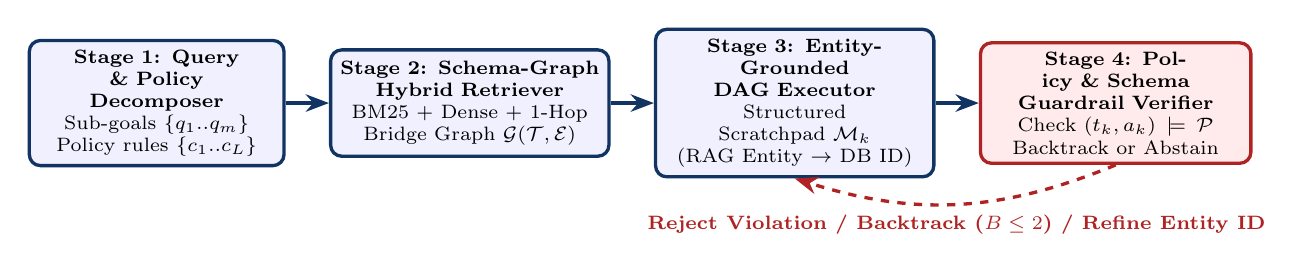
\begin{tikzpicture}[
    node distance=0.45cm and 0.55cm,
    box/.style={rectangle, rounded corners=4pt, draw=navyblue, fill=blue!6, very thick, minimum height=1.35cm, align=center, font=\scriptsize},
    guard/.style={rectangle, rounded corners=4pt, draw=darkred, fill=red!8, very thick, minimum height=1.35cm, align=center, font=\scriptsize},
    arrow/.style={-Stealth, very thick, draw=navyblue}
]
\node[box, text width=3.0cm] (q) {\textbf{Stage 1: Query \& Policy}\\\textbf{Decomposer}\\Sub-goals $\{q_1..q_m\}$\\Policy rules $\{c_1..c_L\}$};
\node[box, text width=3.3cm, right=of q] (ret) {\textbf{Stage 2: Schema-Graph}\\\textbf{Hybrid Retriever}\\BM25 + Dense + 1-Hop\\Bridge Graph $\mathcal{G}(\mathcal{T},\mathcal{E})$};
\node[box, text width=3.3cm, right=of ret] (plan) {\textbf{Stage 3: Entity-Grounded}\\\textbf{DAG Executor}\\Structured Scratchpad $\mathcal{M}_k$\\(RAG Entity $\rightarrow$ DB ID)};
\node[guard, text width=3.2cm, right=of plan] (pol) {\textbf{Stage 4: Policy \& Schema}\\\textbf{Guardrail Verifier}\\Check $(t_k, a_k) \models \mathcal{P}$\\Backtrack or Abstain};

\draw[arrow] (q) -- (ret);
\draw[arrow] (ret) -- (plan);
\draw[arrow] (plan) -- (pol);
\draw[arrow, dashed, draw=darkred, bend left=20] (pol.south) to node[below, font=\scriptsize\bfseries, text=darkred] {Reject Violation / Backtrack ($B \le 2$) / Refine Entity ID} (plan.south);
\end{tikzpicture}
\end{center}
\vspace{-0.15cm}
\begin{columns}[T, onlytextwidth]
\begin{column}{0.32\textwidth}
\begin{block}{\footnotesize 1. Schema Compatibility Graph}
\scriptsize
Offline parsing of $8,000+$ API docstrings builds directed graph $\mathcal{G}(\mathcal{T}, \mathcal{E})$ where $(t_i \rightarrow t_j) \in \mathcal{E}$ if output schema of $t_i$ matches input parameter type of $t_j$. Recovers hidden bridge APIs!
\end{block}
\end{column}
\begin{column}{0.32\textwidth}
\begin{block}{\footnotesize 2. Entity Grounding Scratchpad}
\scriptsize
Maintains structured state $\mathcal{M}_k = \{(\text{mention}, \text{canonical\_id}, \text{source}, \text{type})\}$. Forces lookup API resolution when transferring entities from RAG text to SQL APIs.
\end{block}
\end{column}
\begin{column}{0.32\textwidth}
\begin{alertblock}{\footnotesize 3. Pre/Post Policy Guardrail}
\scriptsize
Evaluates entailment $P_{\text{verify}}(\mathcal{P} \models \neg(t_k, a_k))$ \textbf{before} executing each tool and before emitting $\hat{y}$, directly fixing the $2.4\%$ unanswerable policy bottleneck.
\end{alertblock}
\end{column}
\end{columns}
\end{frame}

% ============================================================================
% SLIDE 6: TECHNIQUES & MODELS TO BE USED
% ============================================================================
\begin{frame}{5. Techniques \& Neural Models to Be Used}
\begin{columns}[T, onlytextwidth]
\begin{column}{0.51\textwidth}
\begin{block}{Neural Models \& Mathematical Formulation}
\footnotesize
\begin{itemize}
    \item \textbf{Hybrid Lexical + Dense Tool Retrieval:}
    $$s_{\text{ret}}(q_i, t) = \lambda \cos(\mathbf{e}(q_i), \mathbf{e}(t)) + (1-\lambda)\,\text{BM25}(q_i, t)$$
    using \texttt{BAAI/bge-large-en-v1.5} (or \texttt{Qwen3-Embedding}) + synthetic query augmentation (Re-Invoke style).
    \item \textbf{Graph-Expanded Cross-Encoder Reranking:}
    Expand top-$k_0$ candidates with $1$-hop bridge neighbors $N_{\mathcal{G}}(t)$ and rerank via \texttt{bge-reranker-v2-m3}.
    \item \textbf{Backbone Agent LLMs:}
    Open-weight tool-calling LLMs (\texttt{Qwen2.5-14B/32B-Instruct}, \texttt{Llama-3.3-70B-Instruct}).
    \item \textbf{Stretch Goal (DPO Alignment):}
    Fine-tune \texttt{Qwen2.5-7B-Instruct} via Direct Preference Optimization (DPO) on verified vs.\ policy-violating traces.
\end{itemize}
\end{block}
\end{column}

\begin{column}{0.46\textwidth}
\begin{exampleblock}{Downloaded vs.\ Implemented by Us}
\footnotesize
\textbf{Downloaded / Existing Components:}
\begin{itemize}
    \item Official \texttt{IBM/vakra} execution harness, SQLite DBs, and ReAct baseline.
    \item Pretrained checkpoints (\texttt{Qwen2.5}, \texttt{Llama-3.3}, \texttt{bge-large}, \texttt{bge-reranker}).
\end{itemize}
\vspace{0.15cm}
\textbf{Original Modules Implemented From Scratch:}
\begin{enumerate}
    \item \textbf{API Compatibility Graph Builder $\mathcal{G}(\mathcal{T}, \mathcal{E})$} \& $1$-hop bridge expansion retriever.
    \item \textbf{Entity-Grounded DAG Controller} with structured cross-source scratchpad $\mathcal{M}_k$.
    \item \textbf{Pre/Post-Execution Policy Verifier} with local backtracking ($B \le 2$ retries) and calibrated abstention threshold $\tau_{\text{safe}}$.
\end{enumerate}
\end{exampleblock}
\end{column}
\end{columns}
\end{frame}

% ============================================================================
% SLIDE 7: DATASETS & QUANTITATIVE EVALUATION METRICS
% ============================================================================
\begin{frame}{6. Dataset(s) \& Quantitative Performance Evaluation Metrics}
\begin{columns}[T, onlytextwidth]
\begin{column}{0.46\textwidth}
\begin{block}{VAKRA Benchmark Dataset (\texttt{ibm-research/VAKRA})}
\footnotesize
\begin{itemize}
    \item \textbf{Executable APIs:} \textbf{8,000+ Python functions} across \textbf{62 enterprise domains} (adapted from BIRD-SQL, Live API-Bench, Wikidata5M).
    \item \textbf{Unstructured Corpora:} Domain-aligned document collections (ClapNQ + enterprise docs) for RAG.
    \item \textbf{Task Splits:}
    \begin{itemize}
        \footnotesize
        \item \textit{Subtasks 1 \& 2:} Single-hop \& Compositional BI API slices ($150+$ candidate tools per domain slice).
        \item \textit{Subtask 3:} Multi-Hop Structured API chains ($2\text{--}7$ hops).
        \item \textit{Subtask 4:} \textbf{664 Multi-Source Samples} (\textbf{420} unconstrained + \textbf{244} policy-constrained; $90\%$ IAA, $96\%$ high-quality human validation).
    \end{itemize}
\end{itemize}
\end{block}
\end{column}

\begin{column}{0.51\textwidth}
\begin{alertblock}{Quantitative Evaluation Metrics \& Baseline Targets}
\footnotesize
\begin{enumerate}
    \item \textbf{Trajectory Execution Accuracy (\texttt{Exec-Acc}):}
    Deterministic replay match of live DB and retrieval states against reference execution graphs.
    \item \textbf{Final Answer Accuracy \& Token-Level F1:}
    Exact match and F1 on synthesized final responses.
    \item \textbf{Tool Selection Recall@$K$ \& F1 (Subtask 2):}
    Accuracy of retrieving gold APIs from $150+$ domain candidates.
    \item \textbf{Policy Compliance Rate \& Abstention F1 (Subtask 4):}
    Correctly blocking restricted tools and abstaining on unanswerable queries ($244$ policy samples).
    \item \textbf{Efficiency Metrics:} Avg.\ API calls \& tokens per trajectory.
\end{enumerate}
\vspace{0.05cm}
\textbf{Published Baseline Scores to Beat (Naik et al., 2026):}
\begin{itemize}
    \scriptsize
    \item Single-Hop: \textbf{70.4\%} $\rightarrow$ Compositional BI: \textbf{50--51\%} $\rightarrow$ Unanswerable Policy: \textbf{2.4\%} (Target: $>60\%$ via Policy Verifier).
\end{itemize}
\end{alertblock}
\end{column}
\end{columns}
\end{frame}

% ============================================================================
% SLIDE 8: THANK YOU & Q&A
% ============================================================================
\begin{frame}
\centering
\vspace{0.8cm}
{\Huge \textbf{Thank You!}}\\[0.4cm]
{\Large \textcolor{navyblue}{\textbf{Questions \& Discussion (5 Minutes)}}}\\[0.8cm]

\begin{columns}[T, onlytextwidth]
\begin{column}{0.85\textwidth}
\centering
\begin{block}{\centering Project Summary}
\footnotesize
\textbf{Task:} SemEval-2027 Task 11 (VAKRA-Advanced) --- All 4 Subtasks ($8,000+$ APIs, $62$ Domains)\\
\textbf{Core Innovation:} \textbf{PV-VAKRA} (Schema-Graph Hybrid Retrieval + Cross-Source Entity Scratchpad + Pre-Execution Policy Guardrail Verifier)\\
\textbf{Key Goal:} Overcome ReAct's $>50\%$ multi-hop degradation and $2.4\%$ policy-constrained bottleneck.
\end{block}
\end{column}
\end{columns}
\end{frame}

\end{document}
